\documentclass[8pt]{extarticle}
\title{Econ 250 HW 8}
\author{Avinash Iyer}
\date{November 2, 2022}

%font setup
%
%\usepackage[math]{anttor}

%paper setup
\usepackage{geometry}
\geometry{letterpaper, portrait, margin=1in}
\usepackage{fancyhdr}

%symbols
\usepackage{amsmath}
\usepackage{amssymb}
\usepackage{hyperref}
\usepackage{gensymb}

\usepackage[T1]{fontenc}
\usepackage[utf8]{inputenc}

%chemistry stuff
\usepackage[version=4]{mhchem}
\usepackage{chemfig}

%plotting
\usepackage{pgfplots}
\usepackage{tikz}

%\usepackage{natbib}

%graphics stuff
\usepackage{graphicx}
\graphicspath{ {./images/} }

%a useful command
\newcommand{\plain}[1]{\textrm{#1}}

%code stuff
%when using minted, make sure to add the -shell-escape flag
%you can use lstlisting if you don't want to use minted
%\usepackage{minted}
%\usemintedstyle{pastie}
%\newminted[javacode]{java}{frame=lines,framesep=2mm,linenos=true,fontsize=\footnotesize,tabsize=3,autogobble,}
%\newminted[cppcode]{cpp}{frame=lines,framesep=2mm,linenos=true,fontsize=\footnotesize,tabsize=3,autogobble,}

\usepackage{listings}
\usepackage{color}
\definecolor{dkgreen}{rgb}{0,0.6,0}
\definecolor{gray}{rgb}{0.5,0.5,0.5}
\definecolor{mauve}{rgb}{0.58,0,0.82}

\lstset{frame=tb,
	language=Java,
	aboveskip=3mm,
	belowskip=3mm,
	showstringspaces=false,
	columns=flexible,
	basicstyle={\small\ttfamily},
	numbers=none,
	numberstyle=\tiny\color{gray},
	keywordstyle=\color{blue},
	commentstyle=\color{dkgreen},
	stringstyle=\color{mauve},
	breaklines=true,
	breakatwhitespace=true,
	tabsize=3
}
\pagestyle{fancy}
\fancyhf{}
\rhead{Avinash Iyer}
\lhead{Econ 250 HW 8}
\begin{document}{
\maketitle
\section*{Conceptual Questions}
\begin{itemize}
	\item \textbf{True}: Since Heloise and Abelard are profit maximizing firms in a perfectly competitive environment, each will produce enough units until the marginal cost equals the average total cost. Since the average total cost for Heloise is half that of Abelard, the marginal letter that Heloise produces will cost half that of the marginal letter that Abelard produces.
	\item \textbf{False}: If, in the short run, Prianca is not operating, then it means that the prevailing market price is below the average variable cost, and since both Cleo and Prianca have the same average variable cost, this means Cleo is also facing the same average variable cost and prevailing market price, so Cleo must also shut down.
\end{itemize}
\section*{Producer Comparisons}
\begin{itemize}
	\item \textbf{True}: Since both Billy and Tommy are operating in a perfectly competitive market with a prevailing market price, their marginal unit of output will occur when marginal revenue equals marginal cost, meaning that the marginal cost must be equal to the market price for both, meaning both are equal.
	\item \textbf{False}: Since Billy's average variable cost is higher than Tommy's, and average variable cost is dependent on marginal cost, and their marginal cost at ideal output is the same, Billy's producer surplus must be below Tommy's.
\end{itemize}
\begin{center}
	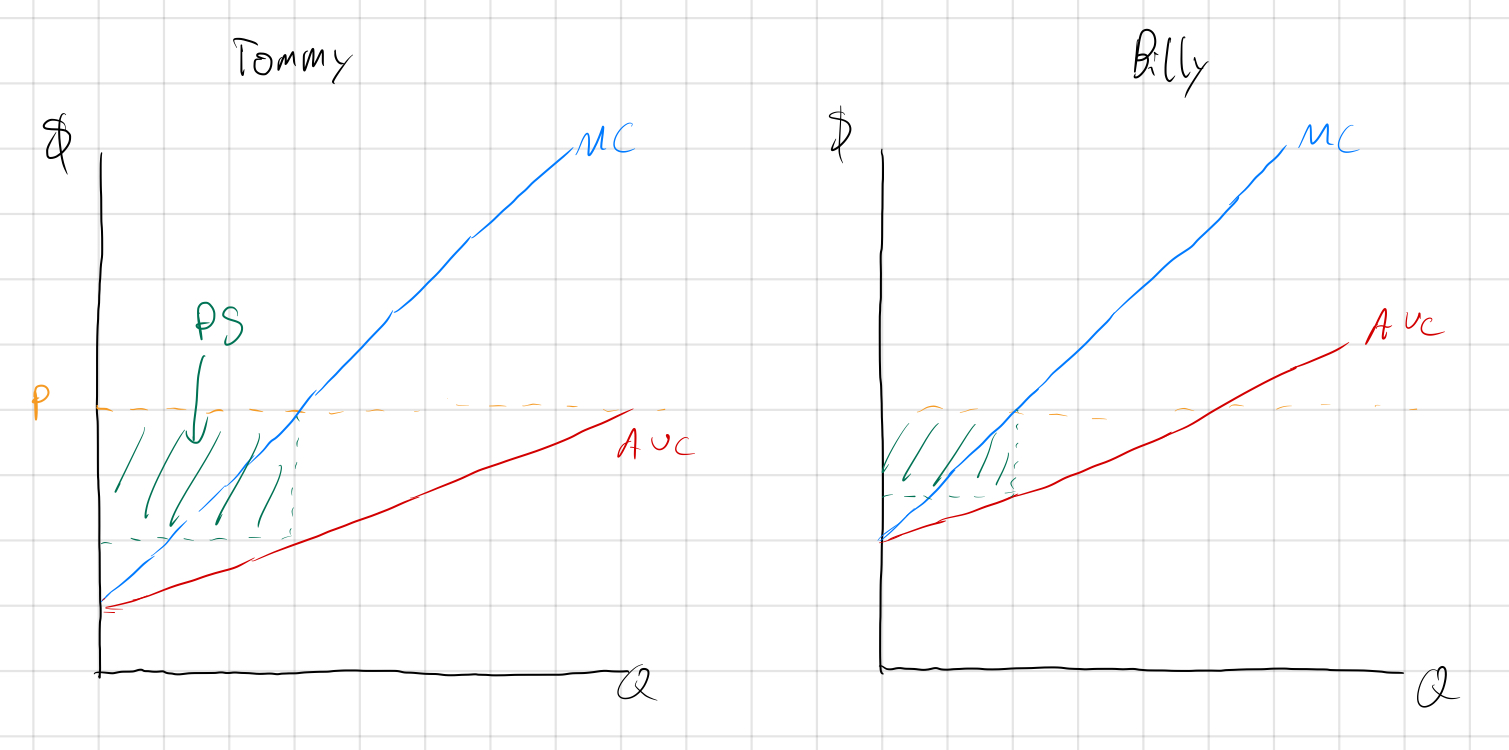
\includegraphics[width=10cm]{HW8Q2B}
\end{center}
\section*{Long Run Profit}
\begin{align*}
	Q &= \sqrt{K} + 3\sqrt{L} \\
	MRTS_{KL} &= \frac{\frac{1}{2\sqrt{K}} }{\frac{3}{2\sqrt{L}}} \\
	&= \frac{\sqrt{L}}{3\sqrt{K}}\\
	\frac{\sqrt{L}}{3\sqrt{K}} &= \frac{25}{150} \\
	\sqrt{L} &= \frac{\sqrt{K}}{2} \\
	Q &= \frac{5\sqrt{K}}{2} \\
	K &= \frac{4Q^2}{25}\\
	L &= \frac{Q^2}{25}\\
	TC &= (25)\left(\frac{4Q^2}{25}\right) + (150)\left(\frac{Q^2}{25}\right) \\
	&= 10Q^2\\
	ATC &= 10Q\\
	MC &= 20Q\\
	P &= 20Q \\
	\pi &= (P - ATC)(Q) \\
	10 &= (20Q - 10Q)(Q) \\
	Q &= 1\\
	P &= \boxed{10}
\end{align*}

\section*{Deriving Short Run Supply}
\subsection*{Part A}
\begin{align*}
	TC &= 32 + 2Q^2\\
	ATC &= 32/Q + 2Q \\
	MC &= 4Q\\
	ATC &= MC \\
	32/Q + 2Q &= 4Q\\
	32/Q &= 2Q \\
	Q &= 4\\
	MC^{*} &= 16 \\
	Q_{S,~\textrm{\tiny firm}} &= \begin{cases}
		0, & P<16 \\
		[0,4], & P=4 \\
		P/4, & P>4
	\end{cases}
\end{align*}
\subsection*{Part B}
\[
Q_{S\textrm{\tiny, market}}\begin{cases}
	0, & P<8\\
	[0,160], & P = 16 \\
	10P, & P\geq 16
\end{cases}
\]
\subsection*{Part C}
\begin{align*}
	10P &= 200-10P \\
	P &= 20 \\
	Q_{\textrm{\tiny market}} &= 200 \\
\end{align*}
	
\subsection*{Part D}
\begin{align*}
	Q_{S,~\textrm{\tiny firm}} &= 5 \\
	ATC &= 32/5 + 2(5) \\
	&= 16.4 \\
	P &= 20
\end{align*}
Since $P > ATC$, each firm \textbf{should} operate in the long run.
\section*{Short Run: Connection Production Function and Markets}
\begin{align*}
	Q &= \sqrt{K}\sqrt{L} \\
	MRTS_{KL} &= \frac{\frac{\sqrt{L}}{2\sqrt{K}}}{\frac{\sqrt{K}}{2\sqrt{L}}} \\
	&= \frac{L}{K} \\
	\frac{L}{K} &= \frac{1000}{15} \\
	L &= \frac{1000K}{15}\\
	L &= \frac{1000(5)}{15} \\
	L &= \frac{1000}{3}\\
	Q &= \sqrt{(5)\left(\frac{1000}{3}\right)} \\
	Q &= 40.8 \\
	40.8 &= 500-8P \\
	P &= 57.4
\end{align*}
\section*{Short Run, Mixed Supplier Types}
\subsection*{Part A}
\begin{center}
	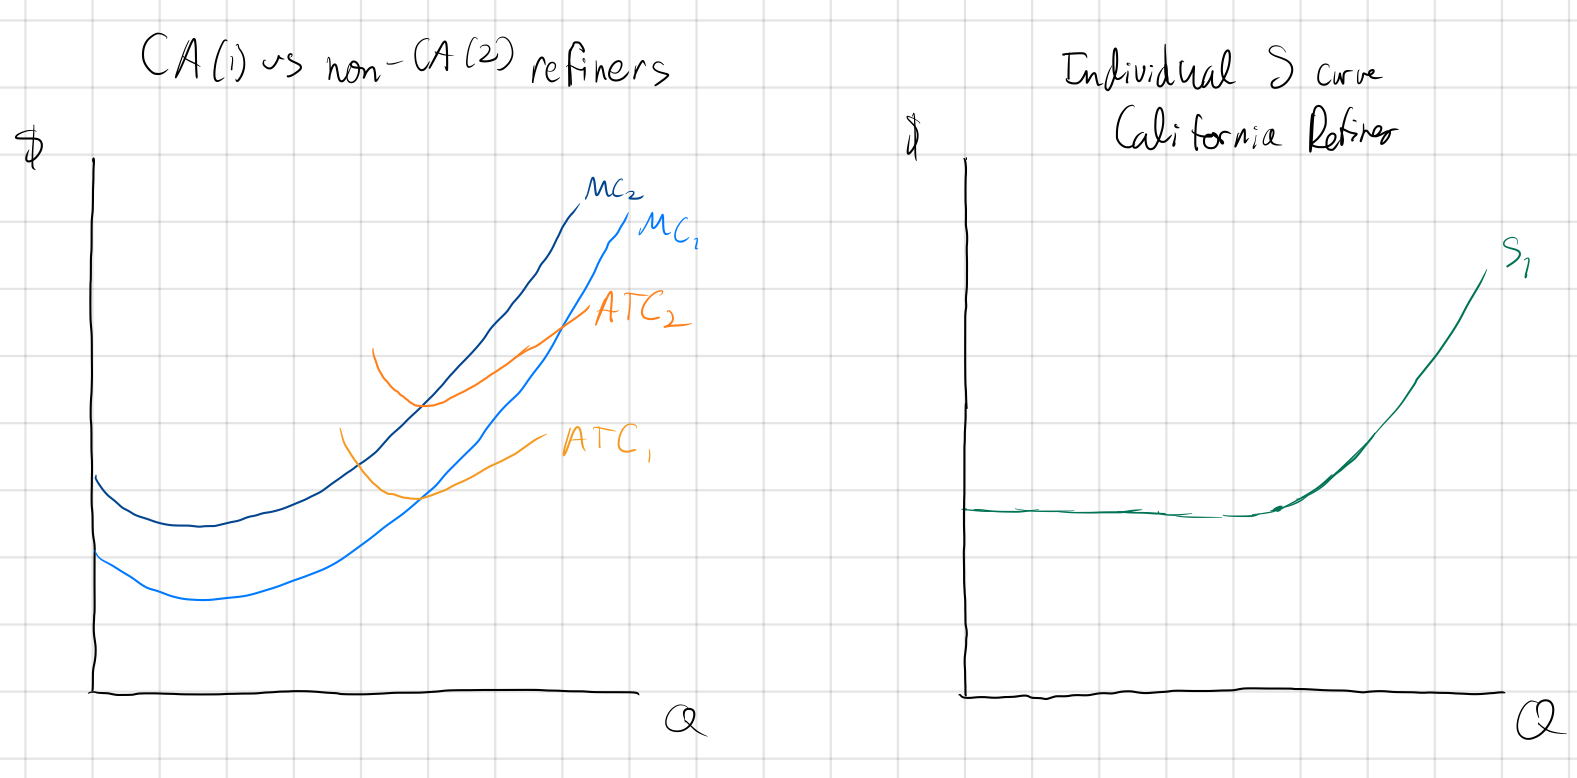
\includegraphics[width=10cm]{HW8Q6A}
\end{center}
\subsection*{Part B}
\begin{center}
	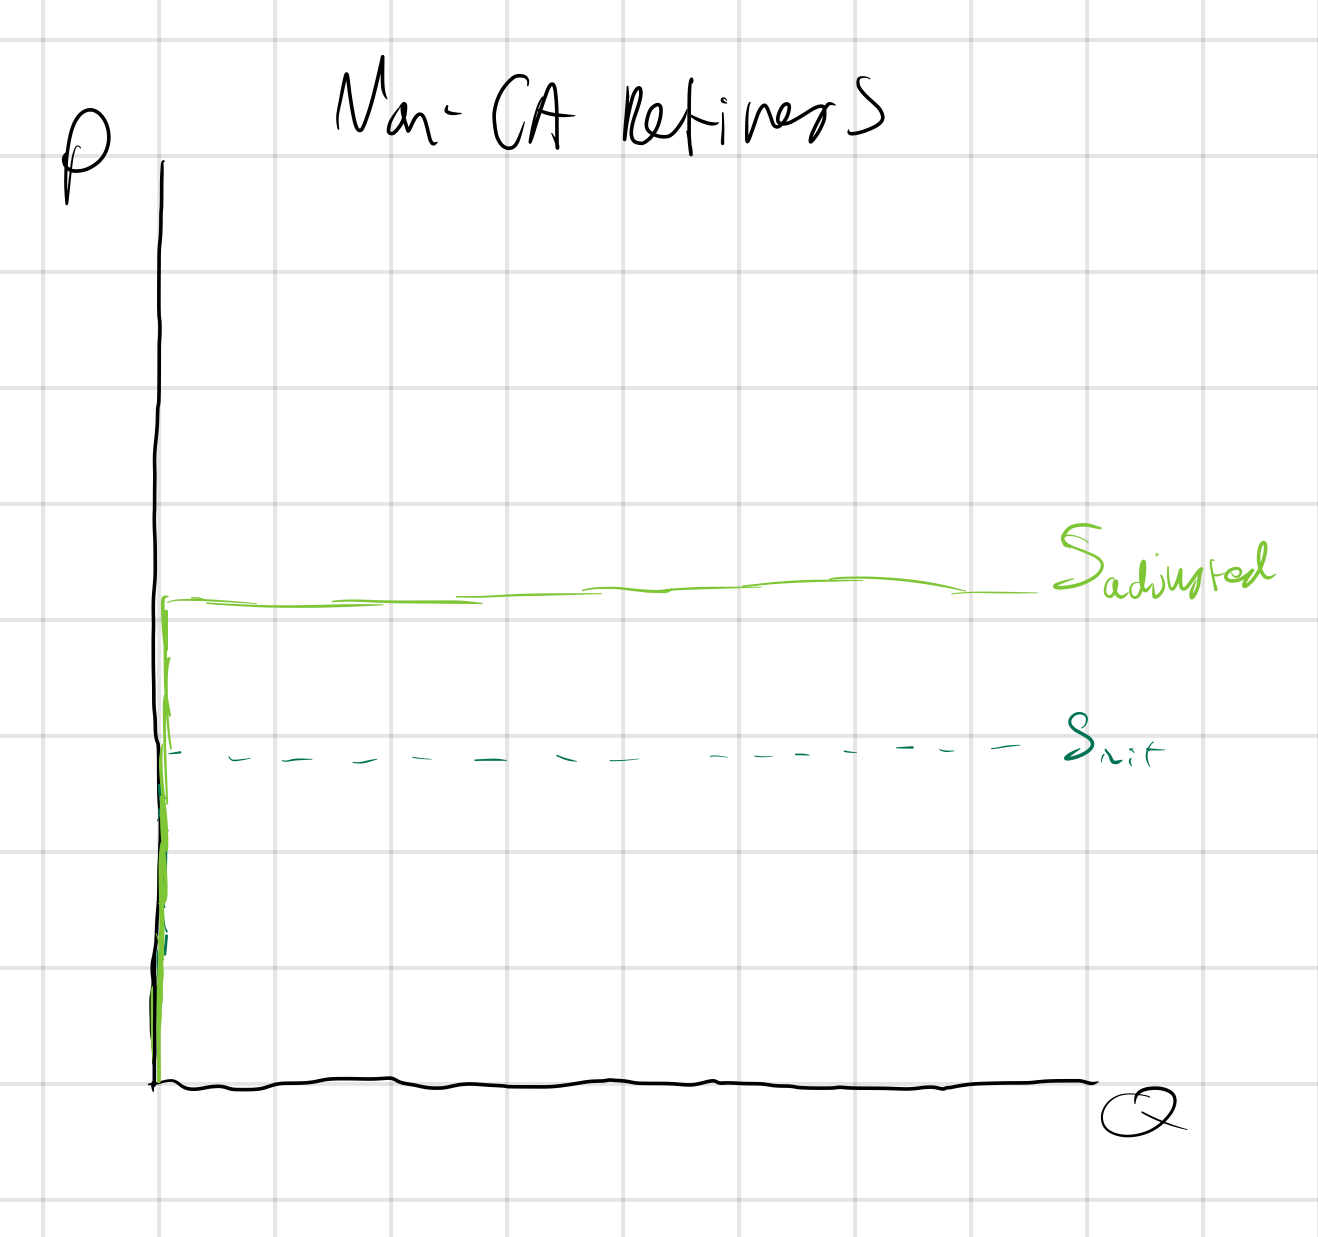
\includegraphics[width=10cm]{HW8Q6B}
\end{center}
\subsection*{Part C}
\begin{center}
	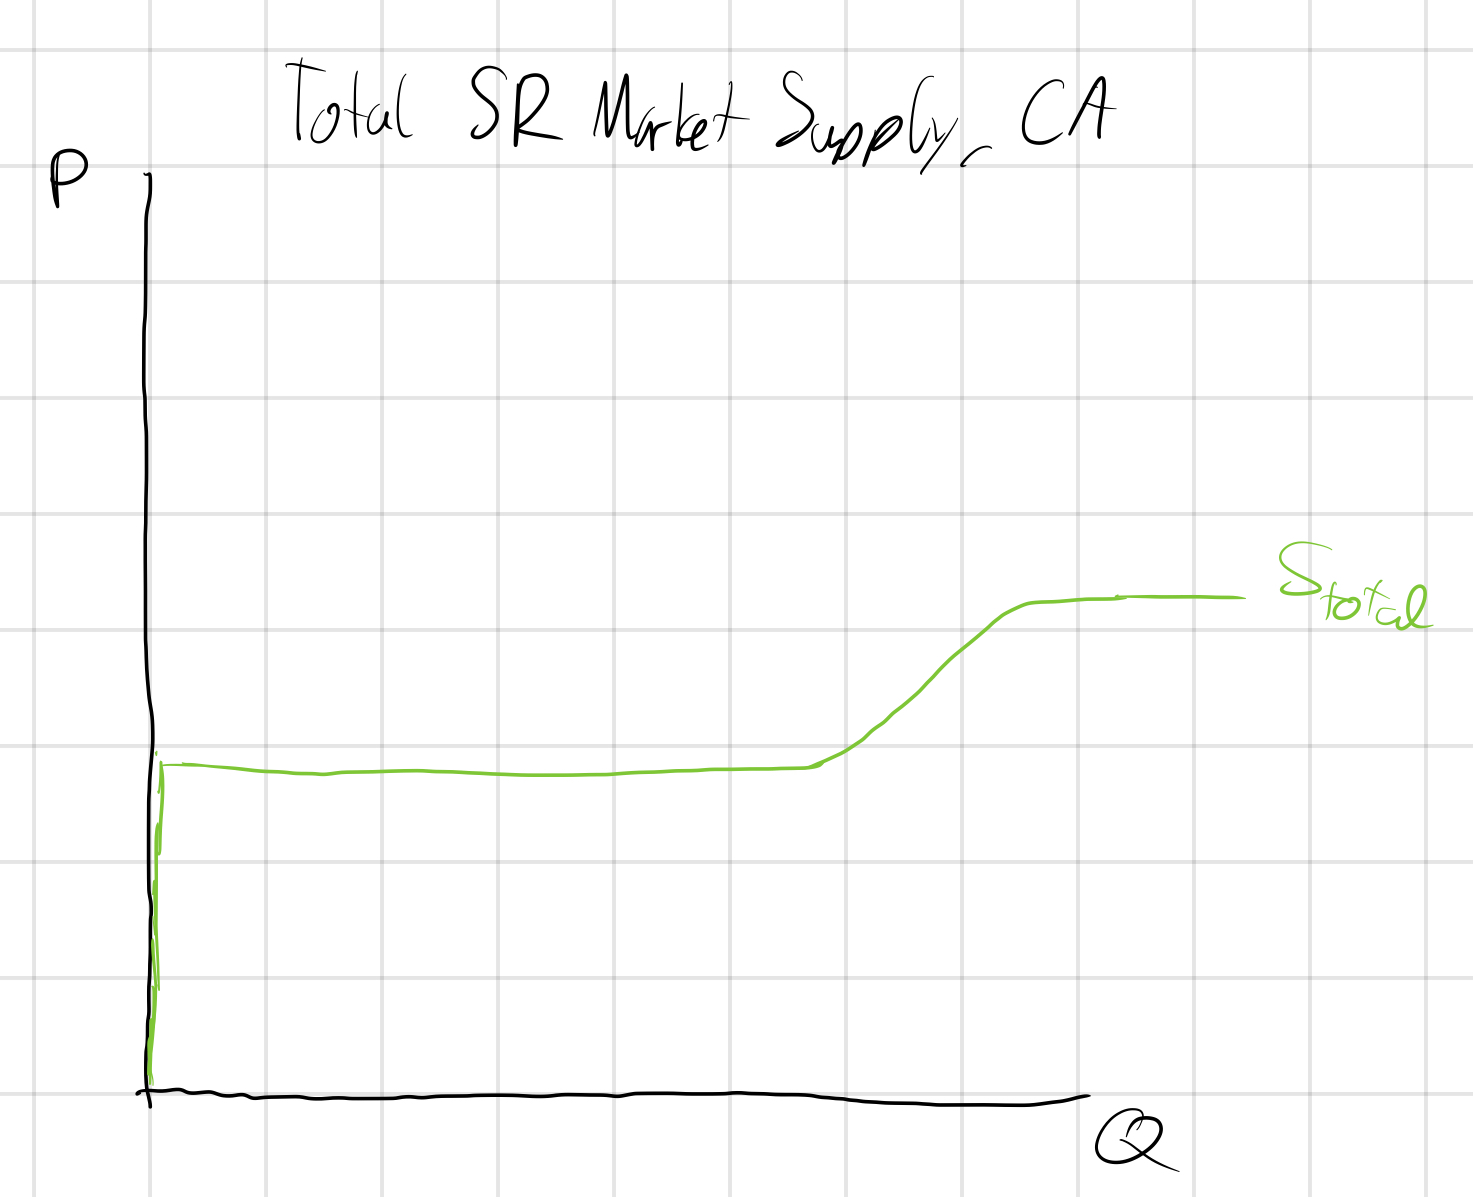
\includegraphics[width=10cm]{HW8Q6C}
\end{center}
\subsection*{Part D}
As California refineries are shut down, the market supply curve from California firms starts shifting inward, until the only refineries producing gasoline are from outside California, which are 10 cents more expensive than refineres producing oil inside California, meaning the maximum possible price increase is 10 cents.
\section*{Long Run Equilibrium Changes}
\begin{center}
	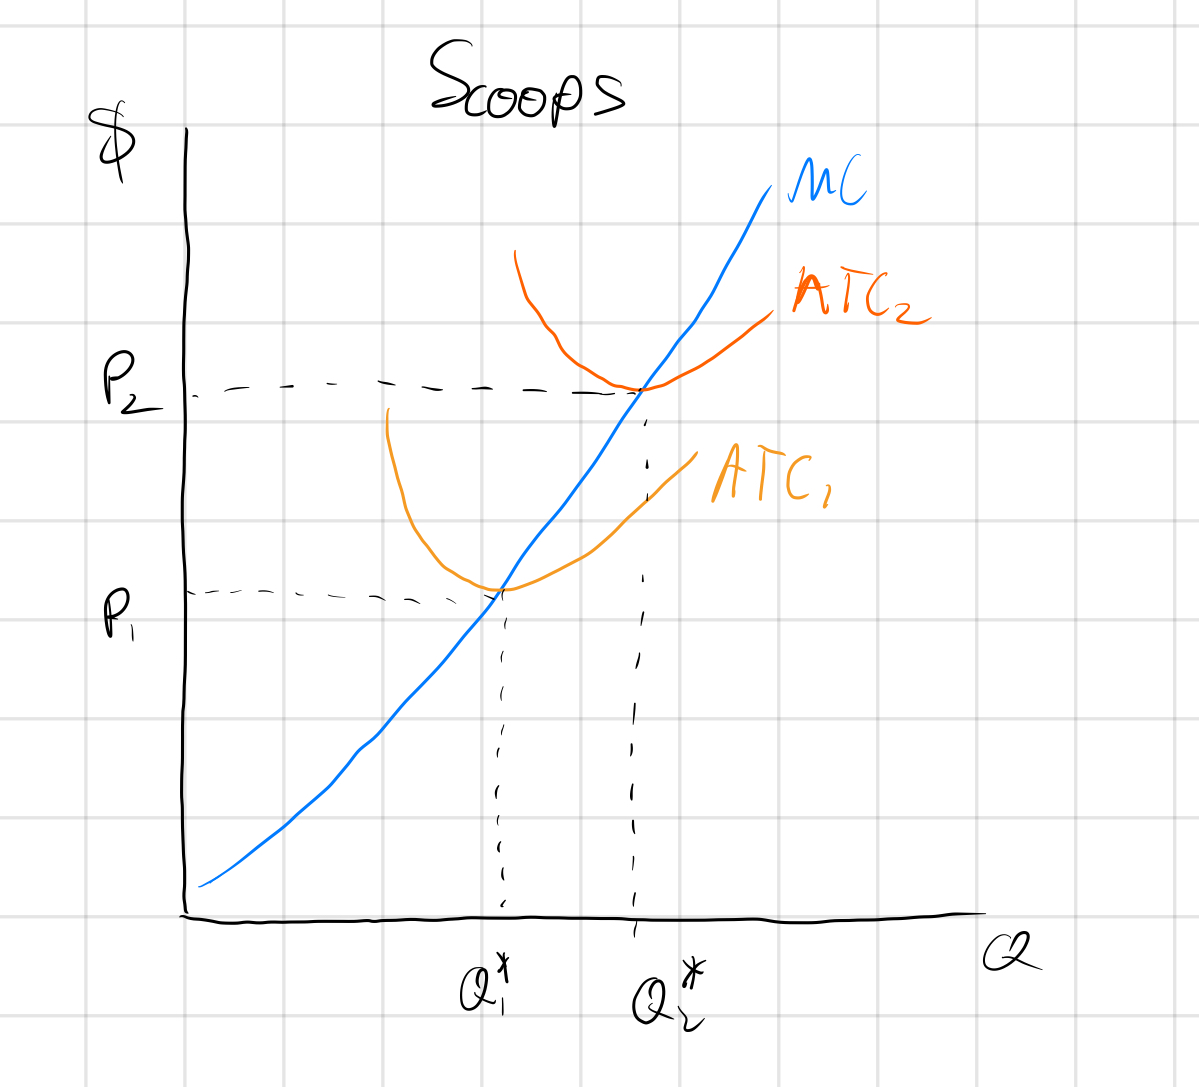
\includegraphics[width=10cm]{HW8Q7}
\end{center}
Because the lump sum tax only affects the total cost rather than the marginal cost, the quantity that Scoops produces \textit{increases}, so the statement is \textbf{false}. Additionally, since in long run equilibrium, Scoops produces zero profits, Scoops is neither better nor worse off.
\section*{Long Run with Mixed Producers and Economic Rent}
\subsection*{Part A}%
\begin{align*}
	LATC_{E} &= 200/Q + Q \\
	LMC_{E} &= 2Q \\
	2Q &= 200/Q + Q \\
	Q &= 200/Q \\
	Q &= 10\sqrt{2}\\
	P &= 20 \sqrt{2}\\
	Q_{S,E} &= \begin{cases}
		0, & P < 20\sqrt{2}\\
		[0,10\sqrt{2}], & P = 20\sqrt{2} \\
		P/2, &P>20\sqrt{2}
	\end{cases}
\end{align*}
\subsection*{Part B}
\begin{align*}
	LATC_{A} &= 200/Q + 2Q \\
	MC_{A} &= 4Q \\
	4Q &= 200/Q + 2Q \\
	Q &= 10\\
	P &= 40\\
	Q_{S,A} &= \begin{cases}
		0, &P<40 \\
		[0,10], &P=40\\
		P/4, & P>40
	\end{cases}
\end{align*}
\subsection*{Part C}
Since there are two different minima for long run average total cost depending on whether the firm has an exceptional manager or an average manager, we cannot know the long run equilibrium price because we don't know whether the market demand only satisfies for firms with exceptional managers or ordinary managers.
\subsection*{Part D}
\begin{align*}
	Q_{S,E} &= \begin{cases}
		0, & P < 20\sqrt{2}\\
		[0,10\sqrt{2}], & P = 20\sqrt{2} \\
		P/2, &P>20\sqrt{2}
	\end{cases} \\
	Q_{S,M,E} &= \begin{cases}
		0, & P<20\sqrt{2} \\
		[0,500\sqrt{2}], &P = 20\sqrt{2} \\
		25P, & P>20\sqrt{2}
	\end{cases}
\end{align*}
If we assumed the market was entirely made of exceptional managers, we would get that $25P = 8000-100P$, or $P = 64$, which is higher than the minimum of the long run average total cost for the firms with average managers.
\subsection*{Part E}
The long run equilibrium price will be $40$, as that is the minimum of the long run average total cost for the firms with average managers.
\subsection*{Part F}
The quantity produced at $P = 40$ is $Q = 8000-(100)(40) = 4000$. The exceptional firms will produce a total of $25P = 1000$ ice creams, meaning that the other $3000$ ice creams are produced by firms with average managers. Since each firm produces $10$ ice creams, this means there are $\boxed{300}$ firms with average managers.
\subsection*{Part G}
The firms with average managers will yield $0$ profits as is consistent with long run equilibrium.
\subsection*{Part H}
The firms with exceptional managers will obtain profits of $(P-ATC)(Q) = (40 - 20)(20) = 400$ per firm, which is equal to the economic rent the manager is generating for the firm.
\section*{Long Run with Mixed Producers}
\begin{align*}
	LRTC_{W} &= 30Q^2 - 600Q + 3000 \\
	ATC &= 30Q - 600 + 3000/Q \\
	MC &= 60Q - 600 \\
	30Q - 600 + 3000/Q &= 60Q - 600 \\
	30Q &= 3000/Q \\
	Q &= 10 \\
	P &= 0\\
	Q &= 10 + \frac{P}{60}  \\
	Q_{W\textrm{\tiny , ind}} &= 10 + \frac{P}{60} \\
	Q_{W \textrm{\tiny, market}} &= 1200 + 2P \\
	\\
	ATC_{O} &= 30Q - 600 + 3000/Q + 40 \\
	&= 30Q - 560 + 3000/Q \\
	MC_{O} &= 60Q - 560 \\
	30Q - 560 + 3000/Q &= 60Q - 560 \\
	Q &= 10 \\
	P_O &= 40 \\
	\\
	1200 + 2P &= 2220-28P \\
	P &= 34
\end{align*}
Since $P^{*} < P_{O}$, where $P_O$ is the threshold price for outside firms to enter the Westview market, \textbf{zero} outside firms enter the market.
}\end{document}